\documentclass{article}
\usepackage[utf8]{inputenc}
\usepackage[T1]{fontenc}
\usepackage{booktabs}
\usepackage{xcolor}
\usepackage{fontawesome5}
\usepackage{geometry}
\usepackage{array}
\usepackage{helvet}
\usepackage{titlesec}
\usepackage{parskip}
\usepackage{mdframed}
\usepackage{hyperref}
\usepackage{ragged2e}
\usepackage{graphicx}
\usepackage{ccicons}
\usepackage{fancyhdr}
\usepackage{lmodern}
\usepackage[export]{adjustbox}

% Meta-Informationen für den PDF-Export
\hypersetup{
    pdftitle={Kursabschluss in Moodle},
    pdfauthor={Christian-Maximilian Steier},
    pdfsubject={Kursabschluss und bedingte Verfügbarkeit in Moodle},
    pdfkeywords={Moodle, Kursabschluss, Voraussetzungen, Christian-Maximilian Steier},
    colorlinks=true,
    linkcolor=customred,
    urlcolor=customred,
    pdfborderstyle={/S/U/W 1}
}

\renewcommand{\familydefault}{\sfdefault}

% Keine Worttrennung
\tolerance=1
\emergencystretch=\maxdimen
\hyphenpenalty=10000
\hbadness=10000
\raggedright

\geometry{a4paper, margin=2.5cm}
\definecolor{customred}{RGB}{230, 0, 40}
\definecolor{lightred}{RGB}{255, 235, 238}
\definecolor{lightblue}{RGB}{235, 245, 255}
\definecolor{lightgray}{RGB}{245, 245, 245}
\definecolor{ccboxborder}{RGB}{200, 200, 200}
\definecolor{ccboxbg}{RGB}{245, 245, 245}

% Titelgestaltung
\titleformat{\section}
  {\normalfont\Large\bfseries\color{customred}}
  {}{0em}{}[\vspace{-0.5em}\rule{\textwidth}{0.5pt}]

% Fußzeile
\pagestyle{fancy}
\fancyhf{}
\renewcommand{\headrulewidth}{0pt}
\fancyfoot[C]{
\ccby{}\quad Dieses Dokument wurde erstellt von \textbf{ZWEK} der Hochschule Düsseldorf und steht unter der Lizenz \textbf{CC BY 4.0}.  
Weitere Informationen: \url{https://creativecommons.org/licenses/by/4.0/}\\
\textsf{\small{Stand: April 2025 • Moodle Version 4.5}}}
\fancyfoot[R]{\textsf{\thepage}}

% Gemeinsame Breite
\newlength{\commonwidth}
\setlength{\commonwidth}{16cm}

% Modernisierte CC-Box
\newenvironment{ccbox}{%
  \begin{center}
  \begin{minipage}{\commonwidth}
  \begin{mdframed}[
    backgroundcolor=ccboxbg,
    linecolor=ccboxborder,
    linewidth=0.8pt,
    roundcorner=5pt,
    leftmargin=0pt,
    innerleftmargin=1em,
    innerrightmargin=1em,
    innertopmargin=0.7em,
    innerbottommargin=0.7em
  ]
  \centering
  \small
}{%
  \end{mdframed}
  \end{minipage}
  \end{center}
}

\begin{document}

% Titel
\begin{center}
\textbf{\textcolor{customred}{\LARGE Kursabschluss \faCheckCircle{} und Voraussetzungen \faLock}}
\end{center}

\vspace{0.5cm}

% Usecase Box
\begin{center}
\begin{minipage}{\commonwidth}
\begin{mdframed}[backgroundcolor=lightgray, linewidth=0pt, roundcorner=5pt]
\textbf{Anwendungsfall:}

Sie möchten sicherstellen, dass Studierende alle erforderlichen Lernaktivitäten abschließen und strukturierte Lernpfade befolgen.

\vspace{0.3cm}

\textbf{Szenarien:}
\begin{itemize}
\item \textbf{Kursabschluss}: Damit können Lernende (und Lehrende) sehen, welche Aktivitäten bereits abgeschlossen wurden und welche noch offen sind. 
\item \textbf{Voraussetzungen}: Inhalte und Aufgaben können abhängig von bestimmten Bedingungen freigeschaltet werden – z.B. "Zeige Kapitel 2 erst, wenn Quiz 1 bestanden wurde."
\end{itemize}
\end{mdframed}
\end{minipage}
\end{center}

\vspace{0.8cm}

\renewcommand{\arraystretch}{1.4}  % Erhöht den Zeilenabstand in der Tabelle
\setlength{\tabcolsep}{8pt}        % Setzt den Spaltenabstand

% Tabelle zentriert mit linksbündigem Text in den Zellen
\begin{center}
\begin{minipage}{\commonwidth}
\begin{tabular}{>{\bfseries\raggedright\arraybackslash}p{3.5cm}>{\raggedright\arraybackslash}p{6cm}>{\raggedright\arraybackslash}p{6cm}}
\toprule
\textcolor{customred}{\textbf{}} 
& \textbf{Aktivitätsabschluss \faCheckSquare} 
& \textbf{Kursabschluss \faGraduationCap} \\
\midrule
Funktion & \faClipboardCheck~Markiert einzelne Aktivitäten als abgeschlossen 
       & \faFlag~Markiert den gesamten Kurs als abgeschlossen \\
\midrule
Voraussetzung 
       & \faCog~Aktivitätsabschluss muss in Kurseinstellungen aktiviert sein 
       & \faClipboardList~Abschlussverfolgung muss aktiviert sein \\
\midrule
Zugriff & \faEdit~Aktivitätseinstellungen → Abschlussbedingungen
        & \faCogs~Kurseinstellungen → Abschlussverfolgung \\
\midrule
Abschlusskriterien & \faList~Anzeigen, Bewertung erhalten, Bestehen, Datum, Aktivität
          & \faLayerGroup~Alle/bestimmte Aktivitäten, manuell, Datum \\
\midrule
Verknüpfung & \faLink~Kann mit Voraussetzungen verknüpft werden 
         & \faCertificate~Kann mit Kurszertifikaten verknüpft werden \\
\midrule
Nutzereinfluss & \faUser~Kann manuell/automatisch erfolgen 
            & \faUsers~Kann von Lehrenden überprüft werden \\
\midrule
Nutzung für & \faRocket~Fortschrittskontrolle einzelner Aktivitäten 
                 & \faMapSigns~Überblick über den Gesamtfortschritt \\
\bottomrule
\end{tabular}
\end{minipage}
\end{center}

\vspace{0.7cm}

% Tipp-Box zentriert mit gleicher Breite wie die Tabelle
\begin{center}
\begin{minipage}{\commonwidth}
\fcolorbox{customred!30}{lightblue!30}{%
    \begin{minipage}{\dimexpr\commonwidth-2\fboxsep-2\fboxrule}
    \raggedright % Inhalt der Box linksbündig
    \textbf{\textcolor{customred}{Tipp:}} Kombinieren Sie Kursabschluss mit bedingter Verfügbarkeit, um Lernpfade zu erstellen. Neue Inhalte werden erst freigeschaltet, wenn vorherige Aktivitäten erfolgreich abgeschlossen wurden – ideal für sequentielles Lernen!
    \end{minipage}%
}
\end{minipage}
\end{center}

\vspace{1.5cm}

\begin{figure}
    \centering
    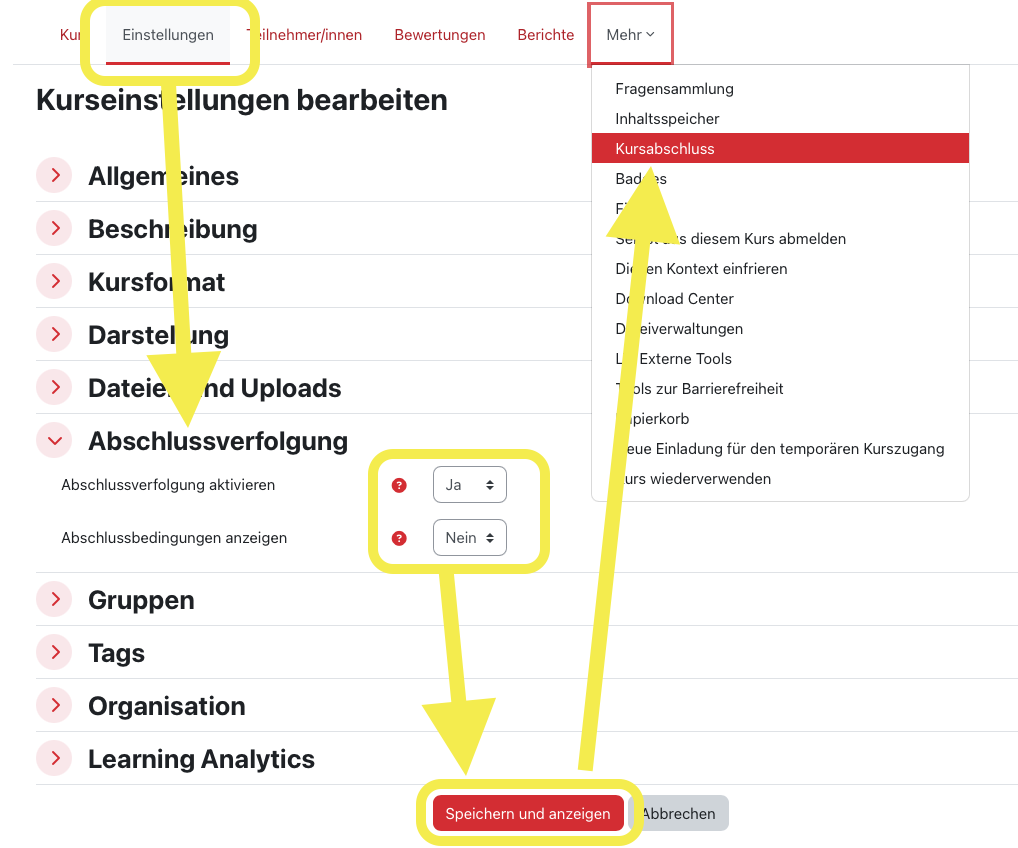
\includegraphics[width=0.9\linewidth]{Bilder/Bild1.png}
    \label{fig:enter-label}
\end{figure}

% Literatur und Links Box zentriert
\begin{center}
\begin{minipage}{\commonwidth}
\begin{mdframed}[
    backgroundcolor=lightgray, 
    linewidth=0pt, 
    roundcorner=5pt,
    innerleftmargin=1em,
    innerrightmargin=1em,
    innertopmargin=0.7em,
    innerbottommargin=0.7em
]
\raggedright % Inhalt der Box linksbündig
\textbf{\textcolor{customred}{Literatur \& Links zum Thema}}
\vspace{0.2cm}

\begin{itemize}
\item \textbf{Offizielle Moodle-Dokumentation:}
\vspace{0.2cm}
  \begin{itemize}
  \item Aktivitätsabschluss: \url{https://docs.moodle.org/de/Aktivit%C3%A4tsabschluss}
  \item Kursabschluss: \url{https://docs.moodle.org/de/Kursabschluss}
  \item Voraussetzungen: \url{https://docs.moodle.org/de/Voraussetzungen}
  \item Video Aktivitätsabschluss (eng): \url{https://youtu.be/oj_c9ykCPgI?si=YqHgcrHHg8j8QEHz}
  \end{itemize}
\vspace{0.5cm}

\item \textbf{Andere Quelle:}
\vspace{0.2cm}
  \begin{itemize}
  \item Aktivitäts- und Kursabschluss setzen: \url{https://academic-moodle-cooperation.org/anleitungen/aktivitats-und-kursabschluss/}
  \item Kursabschluss: \url{https://kb.el.uni-leipzig.de/books/moodle/page/kursabschluss}
  \end{itemize}
\end{itemize}
\end{mdframed}
\end{minipage}
\end{center}

\end{document}
